\chapter{Introduction}

The goal of the mathematical field of topology is to identify properties of systems which are invariant to continuous deformations. Its applications to theoretical physics have traditionally been limited to high-energy physics \cite{Simon_history}, but interest in topological condensed-matter physics has surged in recent decades. Beginning with the discovery of the integer quantum Hall effect in 1980---for which Klaus von Klitzing was awarded the Nobel Prize in Physics \cite{Nobel_1985}---it was realised that states of matter exist which are electrically insulating in the bulk, but which cannot be continuously transformed into a conventional insulator; see Figure~\ref{fig:topo-insulators}. These features have turned out to be well described using tools from topology, earning such materials the name of topological insulators.
\begin{figure}[htb!]
	\centering
	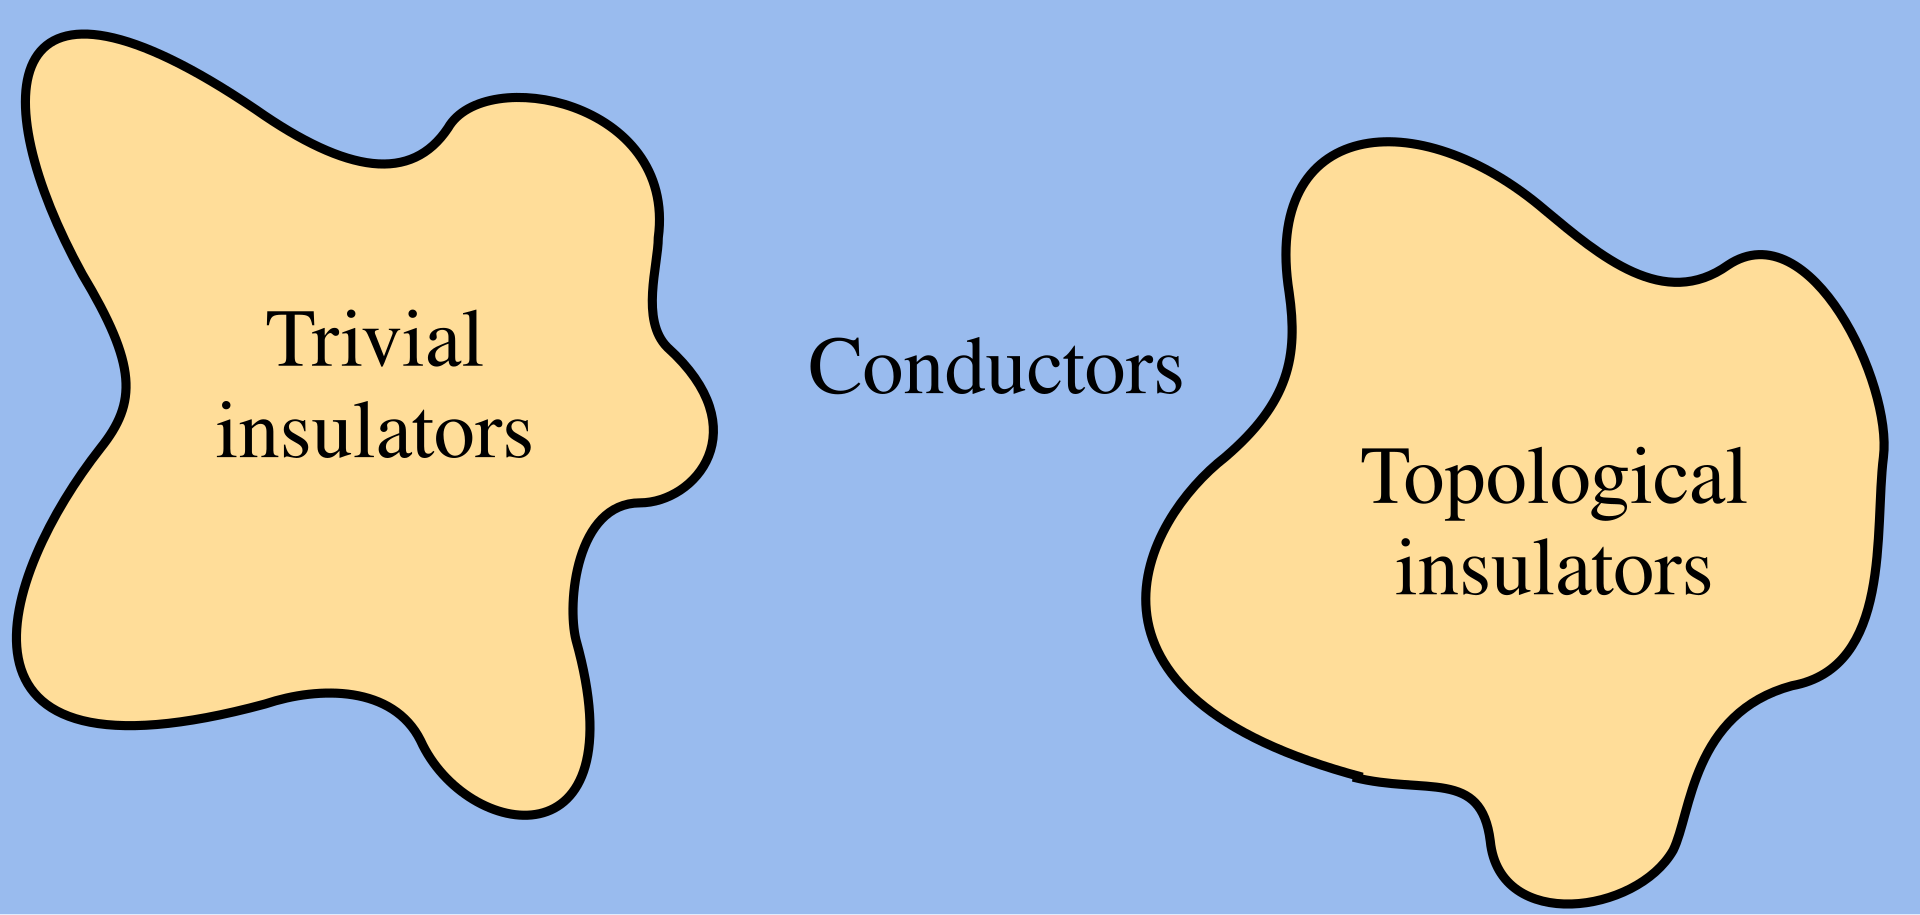
\includegraphics[width=.7\linewidth]{Images/topo-insulators}
	\caption{Schematic phase diagram showing how different types of materials relate. Topological insulators occupy a separate region in phase space from regular insulators, meaning that a Hamiltonian associated with either one cannot be continuously transformed to that of the other without describing a conductor at some intermediate point.}
	\label{fig:topo-insulators}
\end{figure}

Topological insulators have been shown to be a naturally occurring phenomenon \cite{Gehring_natural-TI,Paz_natural-TI}, and they are host to many interesting properties. Perhaps the most distinctive of these properties is the existence of boundary currents: because a topological insulator cannot be continuously connected to a normal insulating state such as the vacuum, conducting states are forced to appear on its interface. These states are protected by the topology of the system, which makes them highly robust to disorder in many cases---a property which may prove to be valuable in applications such as quantum computing, where sensitivity to disorder is one of the main challenges to overcome.

Since the discovery of topological insulators, the study of topology in matter has become an active and rapidly evolving field, eliciting another shared Nobel Prize in Physics as recently as 2016 \cite{Nobel_2016}. Its realm of applicability has been extended to superconductors \cite{Sato_superconductors}, semimetals \cite{Mathai_math-review} and even fully conducting states in metals \cite{Cheng_metals}. It is the semimetals that we are concerned with in this work; these are materials in which the conducting states disperse around certain specific momenta.

\section{Setting}

The main focus of this thesis is on a three-dimensional class of materials called Weyl semimetals, in which the conducting modes resemble the chiral fermions described by Hermann Weyl in 1929 \cite{Weyl_fermions}. The study of these materials is a relatively recent development, with the name first being coined in 2011 \cite{Wan_WSMs}. Weyl semimetals have since been experimentally realised starting in 2015 \cite{Xu_TaAs,Xu_TaAp,Yang-TaAs,Lv_WSM-TaAs}, and they have been found to have exotic transport properties which may have useful applications \cite{Shekhar_magnetoresistance,Osterhoudt_WSM-photovoltaic,Yang_WSM-photovoltaic}.

The chirality associated with left-handed and right-handed Weyl fermions manifests itself as a topological feature in Weyl semimetals: the momenta at which these Weyl modes appear---the so-called Weyl points---have a topological charge associated with them which determines their chirality. Similar to the way in which one left-handed and one right-handed Weyl fermion are paired in the description of a Dirac fermion, the charges in a Weyl semimetal are subject to a cancellation condition known as the Nielsen--Ninomiya theorem \cite{NielsenNinomiya_I,NielsenNinomiya_II}. Concretely, this theorem acts on the unit cell of the momentum-space reciprocal lattice, known as the Brillouin zone: the statement is that the total chirality of all Weyl points in the Brillouin zone should add up to zero. One physical manifestation of this comes in the form of Fermi arcs, which are conducting surface states that connect the projections of oppositely charged Weyl points; see Figure~\ref{fig:fermi-arcs}.
\begin{figure}[htb!]
	\centering
	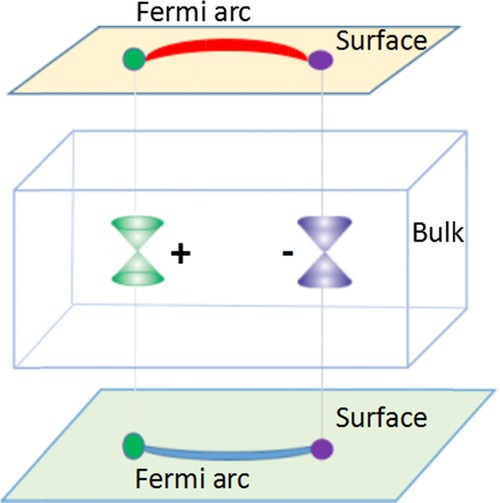
\includegraphics[width=.5\linewidth]{Images/fermi-arcs}
	\caption{Figure from Ref.~\cite{Chi_WSM}. Schematic Weyl semimetal Brillouin zone featuring two oppositely charged Weyl points, whose projections on two different surfaces are shown to be connected by Fermi arcs.}
	\label{fig:fermi-arcs}
\end{figure}

However, recent works have begun to explore materials in which the presence of certain symmetries forces the Brillouin zone to become non-orientable \cite{CYZ_Klein-gauge,TaoYan_acoustic-Klein,Zhu_acoustic-Klein-halfturn,WangZhang_acoustic-Klein-2D}. Non-orientability is a topological property which implies that there is no longer an inherent sense of handedness to a space. A 2024 paper by André Grossi Fonseca, Sachin Vaidya et al. has explored the consequences of applying this non-orientable setting to the intrinsically chiral Weyl semimetals \cite{Fonseca-Vaidya_nonorientable}, and it is this paper that provides the main motivation for this thesis. The authors of Ref.~\cite{Fonseca-Vaidya_nonorientable} find that the Nielsen--Ninomiya theorem no longer straightforwardly applies in the non-orientable case. Instead, the total chirality on the Brillouin zone is only constrained to add to an even number, and Fermi arcs may connect Weyl points with the same chirality under certain circumstances.

However, the description given in Ref.~\cite{Fonseca-Vaidya_nonorientable} is explicitly coordinate dependent, leading to ambiguity in the physical interpretation of the results. Some confusion is also present about the way in which the circumvention of the Nielsen--Ninomiya theorem should be interpreted mathematically.

\section{Research questions}

In this thesis, we aim to provide a deeper understanding of the features found in Ref.~\cite{Fonseca-Vaidya_nonorientable}, both at a mathematical and at a physical level. In particular, we set out to clarify whether the lack of complete charge cancellation can give rise to any phenomenological consequences.

We achieve this by studying non-orientable Weyl semimetals in a more rigorous mathematical framework. To this end, we develop an extension of an existing description in terms of the topological tools of homology and cohomology, first introduced by Varghese Mathai and Guo Chuan Thiang \cite{Mathai_math-review,Mathai_math-paper}. We study how this framework needs to be modified to account for non-orientability, and how the subsequent results differ qualitatively from the orientable setting.

From this more abstract mathematical point of view, we also examine how and to what extent the setting of non-orientable Weyl semimetals can be generalised, both to different non-orientable Brillouin zones and to more general orientation-reversing symmetries.

\section{Outline}

We offer a brief overview here of the organisation of this work. We begin in Chapter~\ref{chap:prerequisites} by introducing some of the prerequisite physical and mathematical concepts. On the physical side, we review some basic aspects of condensed-matter physics, with an emphasis on the core assumptions used in our model. On the mathematical side, we offer a relatively low-level overview of the concepts of homology and cohomology.

Chapter~\ref{chap:topo-states} is a review of different gapped topological states of matter, with an emphasis on those systems which are relevant to the later description of semimetals. Special attention is also paid to the role that symmetries play in determining the topology of a material, with the tenfold classification of symmetry classes taking centre stage.

A review of the theory of Weyl semimetals is provided in Chapter~\ref{chap:WSM}. The first portion of this chapter is dedicated to describing the essential physical properties of these systems, and its remainder delves into the mathematical description in terms of homology and cohomology that is given in Ref.~\cite{Mathai_math-review}.

Chapter~\ref{chap:non-orientable} focuses on non-orientable topology, and it is this chapter that contains the bulk of our results. We begin with a review of the existing literature on non-orientable materials, culminating in a treatment of Ref.~\cite{Fonseca-Vaidya_nonorientable} on Weyl semimetals. We then spend the remainder of the chapter explicating a rigorous framework in which these systems can be studied, and exploring some of the consequences of this description. This part of the work is original.

Finally, the main conclusions of our research are summarised in Chapter~\ref{chap:conclusions}, and some recommendations for further avenues of research are given.